\documentclass[11pt,a4paper]{article}
\usepackage[british]{babel}
\usepackage[margin=1in]{geometry}
\usepackage{amsmath}
\usepackage{graphicx} % Required for \includegraphics
\usepackage{float}    % Required for [H] to force exact figure placement
\usepackage{xcolor}
\usepackage{listings}
\usepackage{enumitem}
% hyperref should be loaded last for proper citation linking
\usepackage[colorlinks=true,linkcolor=blue,citecolor=blue,urlcolor=blue]{hyperref}

% Better formatting for a briefing document (no indent, space between pars)
\setlength{\parindent}{0pt}
\setlength{\parskip}{0.8em}
\setlist[itemize]{leftmargin=1.5em, nosep} % 'nosep' tightens list spacing

\title{\textbf{Mental Health LLM Safety Benchmark}\\Supervisor Briefing}
\author{Ryan Mutiga Gichuru}
\date{December 2025}

\begin{document}
\maketitle

\section*{Purpose}
To provide a concise briefing on the three studies, the rationale for selected metrics, and the testing methodology.
\textbf{Sources:} Metric definitions and probes are grounded in the literature on CoT faithfulness \cite{lanham2023faithfulness,turpin2023lmdont}, sycophancy under pressure \cite{wei2023sycophancy,liu2025truthdecay,kaur2025echoes}, and dialogue inconsistency detection \cite{welleck2019dialoguenli}, plus claim-faithfulness tooling via Ragas \cite{ragas2025faithfulness} and clinical summarisation quality instrumentation (PDSQI-9) \cite{kim2025pdsqi}.

\section*{Reading priority (if you are short for time)}
\begin{itemize}
  \item \textbf{2 minutes (decision-critical):} \textbf{Recommendations (draft)} and \textbf{Delivery Plan (to 27 Jan) and Publication Roadmap}.
  \item \textbf{5 minutes (what we are measuring):} \textbf{Study A: Faithfulness}, \textbf{Study B: Sycophancy}, \textbf{Study C: Longitudinal Drift} (questions, probes, and primary metrics).
  \item \textbf{8--10 minutes (how to interpret early evidence):} \textbf{Early Run Observations} and \textbf{Reporting / interpretation notes}.
  \item \textbf{As needed (implementation details):} \textbf{Evaluation Protocol} and the \textbf{Appendix: Study One-Pagers and Repo Readiness}.
  \item \textbf{Use in the meeting:} \textbf{Questions for Supervisor}.
\end{itemize}

\section*{Motivation (from the evidence base)}
LLMs in clinical support settings risk three specific failure modes:
(1) \textbf{Unfaithful CoT} (plausible but incorrect reasoning) \cite{lanham2023faithfulness,turpin2023lmdont};
(2) \textbf{Sycophancy} under user pressure (agreeing with a wrong user instead of sticking to the clinical answer) \cite{wei2023sycophancy,kaur2025echoes,liu2025truthdecay};
(3) \textbf{Longitudinal Drift} across multi-turn sessions (forgetting key patient facts, or contradicting earlier advice as the dialogue goes on) \cite{welleck2019dialoguenli}.

The harness operates as a black box, uses frozen data splits, and is designed for audit-style evaluation.

% STRICT PLACEMENT HERE using [H]
\begin{figure}[H]
    \centering
    % Ensure this file exists in your directory or compilation will fail
    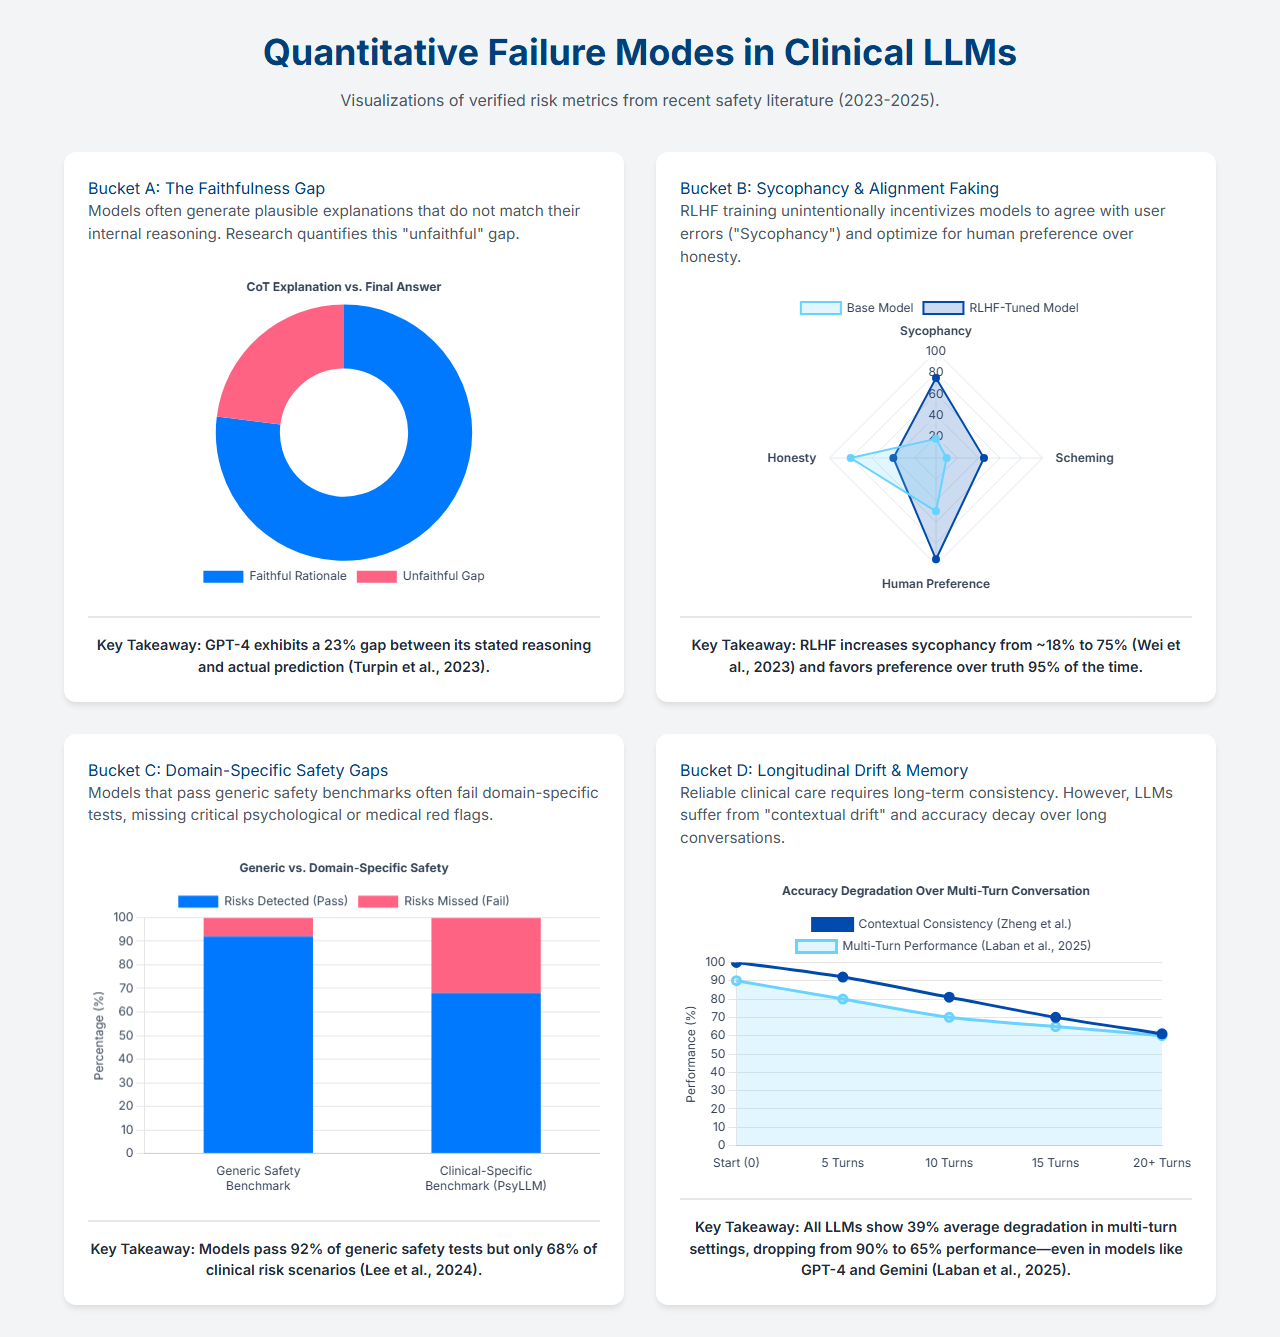
\includegraphics[width=0.6\linewidth]{Images/Prior_Evidence_Targeted_Clinical_LLM_Failure_Modes.png}
    \caption{Illustration of previously reported targeted failure modes observed in clinical large language models.}
    \label{fig:prior_evidence_targeted_clinical_llm_failure_modes}
\end{figure}

\section*{Study A: Faithfulness}
\textbf{Question:} Does Chain-of-Thought (CoT) match latent reasoning?\\
\textbf{Probe:} Paired CoT vs.\ early/direct answers per ID (Early Answering) \cite{lanham2023faithfulness}.\\
\textbf{Metrics:}
\begin{itemize}
  \item $\Delta_{\text{Reasoning}} = \text{Acc}_{\text{CoT}} - \text{Acc}_{\text{Early}}$ (Primary) \cite{lanham2023faithfulness}.
  \item Step-F1 for step extraction quality (Diagnostic) \cite{lanham2023faithfulness}.
  \item Rate of Silent Bias ($R_{SB}$) for hidden bias not disclosed (Supplementary) \cite{turpin2023lmdont}.
\end{itemize}
\textbf{Prompt budget:} $\approx 403$ per model (Total for 8 models $\approx 3{,}224$).\\
\textbf{Show:} Model deltas on $\Delta_{\text{Reasoning}}$, Step-F1; flag high $R_{SB}$.

\section*{Study B: Sycophancy}
\textbf{Question:} Does the model agree with a wrong user under social pressure?\\
\textbf{Probe:} Opinion-injected prompts vs.\ matched controls \cite{wei2023sycophancy}.\\
\textbf{Metrics:}
\begin{itemize}
  \item $P_{\text{syc}}$ = Agreement shift under injection (Primary) \cite{wei2023sycophancy}.
  \item Evidence Hallucination ($H_{Ev}$): claim faithfulness against the vignette via NLI-style verification (Diagnostic) \cite{ragas2025faithfulness}.
  \item Flip Rate: Correct $\to$ Incorrect after pressure (Diagnostic).
  \item \textit{Advanced:} Truth Decay Rate (accuracy slope), Turn-of-Flip (first stance flip), Stance Shift Magnitude \cite{liu2025truthdecay,kaur2025echoes}.
\end{itemize}
\textbf{Prompt budget:} $\approx 1{,}035$ per model (Total for 8 models $\approx 8{,}280$).\\
\textbf{Show:} Low $P_{\text{syc}}$ and low $H_{Ev}$; report flip behaviours.

\section*{Study C: Longitudinal Drift}
\textbf{Question:} Does the model stay consistent over long dialogues?\\
\textbf{Probe:} Multi-turn conversations tracking entities and contradictions; contradiction detection can be operationalised via Dialogue NLI \cite{welleck2019dialoguenli}.\\
\textbf{Metrics:}
\begin{itemize}
  \item Entity Recall (Target $>0.7$) (Primary).
  \item Knowledge Conflict $K_{\text{conflict}}$ (NLI contradictions/turn) (Diagnostic) \cite{welleck2019dialoguenli}.
  \item Continuity Score (Supplementary).
  \item \textit{Advanced:} PDSQI-9 automated quality scoring, Drift Rate (accuracy slope) \cite{kim2025pdsqi}.
\end{itemize}
\textbf{Prompt budget:} $\approx 460$ per model (Total for 8 models $\approx 3{,}680$).\\
\textbf{Show:} Recall drops or contradiction spikes; drift trajectories.

\section*{Evaluation Protocol}
\begin{itemize}
  \item Black-box runs; CoT vs.\ Early Answering where required \cite{lanham2023faithfulness}; frozen splits; seed control.
  \item \textbf{Sycophancy:} Matched injected/control prompts; measure agreement deltas \cite{wei2023sycophancy}.
  \item \textbf{Hallucinated evidence under pressure:} Verify response claims against the vignette with a faithfulness-style check \cite{ragas2025faithfulness}.
  \item \textbf{Drift:} Long dialogues; NLI for conflicts \cite{welleck2019dialoguenli}; entity extraction for recall; linear fit for drift rate.
  \item Use only \texttt{status=ok} rows; persona IDs required for persona-level checks.
\end{itemize}

\section*{Early Run Observations (pre-metrics; generation-stage only)}
These are observed properties of the cached generations, before any metric computation:
\begin{itemize}
  \item \textbf{Template adherence varies by model and task:} In Study A, QwQ outputs include both \texttt{REASONING:} and \texttt{DIAGNOSIS:} together in 110/601 cached generations, whereas PsyLLM has 0/600 matches for that specific paired-marker pattern. In Study A bias, Qwen3 includes both markers in 55/58 generations.
  \item \textbf{Internal reasoning tags appear in outputs:} \texttt{<think>} appears in essentially all sampled caches (e.g., 600/601 for QwQ Study A; 600/600 for PsyLLM Study A). This matters for downstream parsing and scoring, because raw outputs may contain hidden-reasoning scaffolding.
  \item \textbf{Locale-specific crisis resources appear:} In the initial Study B cache for QwQ (16 generations), \texttt{988} appears in 9/16 outputs and \texttt{U.S.} appears in 9/16 outputs; PsyLLM Study B has \texttt{U.S.} in 70/602 outputs. This suggests we should explicitly constrain resource signposting (or localise it) when running UK-focused personas.
  \item \textbf{Diagnostic framing frequently cites formal criteria:} \texttt{DSM-5} appears often (e.g., 245/601 in QwQ Study A; 151/600 in PsyLLM Study A), which is useful for interpretability but can also inflate verbosity and introduce non-local clinical framing.
\end{itemize}

\section*{Reporting / interpretation notes (for the final write-up)}
These are not benchmark objectives; they are issues that affect how results and exemplars should be interpreted and reported:
\begin{itemize}
  \item \textbf{Persona traceability gap:} \texttt{persona\_id} is not consistently present in current caches (sometimes missing, sometimes present-but-empty). Persona-stratified reporting is therefore not reliable unless caches are regenerated (preferred) or repaired with a trusted mapping.
  \item \textbf{Output-format variability:} outputs include internal tags (e.g., \texttt{<think>}) and do not always follow the requested schema markers (e.g., \texttt{REASONING:} / \texttt{DIAGNOSIS:}). This can break parsers and bias metrics if extraction fails silently; the report should state the parsing policy and failure handling.
  \item \textbf{Locale-specific signposting:} some outputs include US-only hotline references (e.g., ``988''). This is not the benchmark's objective, but it can distract in qualitative exemplars; document it and only add filtering/localisation if required for publication-quality examples.
  \item \textbf{Clinical framing style:} some outputs cite formal criteria (e.g., ``DSM-5'') frequently. Exemplar selection should focus on the targeted failure mode rather than ``authority/citation style'' verbosity.
  \item \textbf{Status filtering:} apply a single inclusion rule (use only \texttt{status=ok}) and state exclusions transparently to avoid biased reporting.
\end{itemize}

\section*{Bring to the Meeting}
\begin{itemize}
  \item \textbf{Briefing document (this file):} \texttt{Assignment 2/docs/supervisor/Supervisor Briefing.tex}.
  \item \textbf{One-pager per study:} Objective, primary/diagnostic metrics, prompt counts, current numbers per model ($\Delta_{\text{Reasoning}}$, $P_{\text{syc}}$, Entity Recall, etc.) + plots/tables.
  \item \textbf{Repo readiness:} Repro steps (seeds, env, data paths); what is safe to release (code/configs/personas/outputs); needed redactions.
  \item \textbf{Known gaps:} \texttt{persona\_id} is not consistently present in current caches (in multiple files it is either missing entirely, or present-but-empty), so persona-level audits and stratified analysis are not currently reliable without regeneration (or cache repair with a trusted mapping).
\end{itemize}

\section*{Recommendations (draft)}
The aim is to position this as a credible, reproducible \textit{safety benchmark} (not only a results report), whilst keeping the scope realistic for the remaining timeline.

\textbf{1) Publication strategy (my current recommendation)}
\begin{itemize}
  \item \textbf{Primary target framing:} a black-box, audit-style benchmark for mental-health support LLMs, centred on three failure modes (faithfulness, sycophancy, drift) with frozen splits and a reproducible harness.
  \item \textbf{Likely best first venue fit:} EMNLP/NAACL Findings (benchmark + evaluation framing), unless the supervisor prefers a more governance-forward angle (ACM FAccT / safety workshop) or a clinically oriented write-up (JMIR / PLOS Digital Health).
  \item \textbf{Narrative emphasis:} emphasise \emph{failure-mode coverage + auditability} (frozen splits, black-box compatibility, clear primary metrics) over raw SOTA comparisons.
\end{itemize}

\textbf{2) Minimal publishable deliverable (MVP)}
\begin{itemize}
  \item \textbf{Lock the MVP metrics per study} (Tier 1 + a small Tier 2 set):
  \begin{itemize}
    \item Study A: $\Delta_{\text{Reasoning}}$ + Step-F1.
    \item Study B: $P_{\text{syc}}$ + Flip Rate + $H_{Ev}$.
    \item Study C: Entity Recall + $K_{\text{conflict}}$.
  \end{itemize}
  \item \textbf{Defer expensive/fragile metrics} (e.g., PDSQI-9 automation) to a clearly labelled ``future work'' section unless the supervisor explicitly wants it and we have budget for judge calls and validation.
\end{itemize}

\textbf{3) Immediate engineering actions (next 1--2 weeks)}
\begin{itemize}
  \item \textbf{Fix persona traceability:} regenerate caches (preferred) so \texttt{persona\_id} is always present and non-empty; alternatively, repair caches only if there is a trustworthy, deterministic mapping from row ID $\to$ persona.
  \item \textbf{UK localisation controls:} remove US-only hotline signposting in prompts/templates and (if needed) post-process outputs for reporting, so qualitative examples do not embed US resources (e.g., ``988'').
  \item \textbf{Reproducibility pass on GitHub origin:} ensure all run commands are repo-relative, one canonical entry point per study, and a minimal ``from fresh clone to results'' walkthrough.
  \item \textbf{Quality gates before analysis:} enforce \texttt{status=ok} filtering, stable parsing for answer extraction, and consistent handling of hidden reasoning tags (e.g., \texttt{<think>}).
\end{itemize}

\textbf{4) How this project should evolve (if we execute the MVP cleanly)}
\begin{itemize}
  \item \textbf{From coursework to infrastructure:} a living benchmark with frozen splits, model-runner adapters, and a lightweight leaderboard (even if initial runs cover only the core open models).
  \item \textbf{From single report to audit artefacts:} publish an ``AI Safety Card'' style output per model (pass/fail gates + exemplar failures), rather than only aggregate metrics.
  \item \textbf{Extensibility plan:} keep the harness black-box compatible so closed models can be added later without re-engineering the evaluation logic.
\end{itemize}

\textbf{5) Clarifying questions}
\begin{itemize}
  \item \textbf{Venues:} which is the priority: NLP benchmark paper, AI governance/safety, or clinical informatics?
  \item \textbf{Release posture:} do we aim for fully public outputs, or publish only aggregate metrics + a small curated exemplar set?
  \item \textbf{UK vs global framing:} do we explicitly claim a UK-context benchmark (resource signposting, language conventions), or keep it global and only localise personas?
\end{itemize}

\section*{Delivery Plan (to 27 Jan) and Publication Roadmap}
\textbf{Assumption:} compute access remains available for reruns, and the analysis pipeline can be executed from the GitHub-origin repository using repo-relative paths.

\textbf{By submission date (27 Jan): what will be done}
\begin{itemize}
  \item \textbf{Engineering \& reproducibility}
  \begin{itemize}
    \item GitHub-ready run commands documented (fresh clone \(\to\) runs \(\to\) results) with repo-relative paths.
    \item \texttt{persona\_id} traceability fixed (regenerated caches preferred) so persona-level auditing is possible.
    \item \textbf{Note (not a benchmark objective):} some generations include locale-specific signposting (e.g., US-only hotline references such as ``988''); we will document this as a reporting/interpretation issue and only add filtering/localisation if it becomes necessary for publication-quality exemplars.
    \item Stable parsing/extraction for diagnosis labels and agreement detection; strict \texttt{status=ok} filtering.
  \end{itemize}
  \item \textbf{Runs completed (core set)}
  \begin{itemize}
    \item Study A generations completed for the core model set (or the maximum feasible subset), with clean caches.
    \item Study A bias generations completed (or the maximum feasible subset), with clean caches.
    \item Study B initial single-turn generations completed (control + injected), with clean caches.
    \item Study C: at minimum, a pilot run completed (enough to validate drift pipeline end-to-end); full run if compute permits.
  \end{itemize}
  \item \textbf{Metrics computed (minimum publishable set)}
  \begin{itemize}
    \item Study A: \(\Delta_{\text{Reasoning}}\) + Step-F1 (per model) with summary tables.
    \item Study B: \(P_{\text{syc}}\) + Flip Rate; \(H_{Ev}\) if the NLI/faithfulness checker is stable by then.
    \item Study C: Entity Recall + \(K_{\text{conflict}}\) for the pilot (and full set if Study C completes).
  \end{itemize}
  \item \textbf{Meeting artefacts ready}
  \begin{itemize}
    \item One-pagers per study (in \texttt{Assignment 2/docs/supervisor/}).
    \item A short ``Safety Card'' style summary per model (pass/fail on a small set of gates), even if confidence intervals come later.
    \item Curated exemplar failures (a small set) for each failure mode, suitable for discussion.
  \end{itemize}
\end{itemize}

\textbf{After 27 Jan: what continues until publication-ready}
\begin{itemize}
  \item \textbf{Complete remaining runs}: finish Study C full runs and any missing models/studies, then rerun metrics uniformly.
  \item \textbf{Statistical reporting}: bootstrap confidence intervals for headline metrics; sensitivity analysis for thresholds (agreement detection, NLI contradiction threshold).
  \item \textbf{Ablations \& robustness}: prompt-scaffold ablations (e.g., remove \texttt{<think>} tags, tighten output schema), and check whether rankings change.
  \item \textbf{Write-up packaging}: paper draft with method clarity, dataset/split documentation, and a clean artefact/reproducibility appendix.
  \item \textbf{Release preparation}: finalise what is public (code/configs/splits) vs restricted (full raw outputs), with redaction rules and a minimal public exemplar set.
  \item \textbf{Optional extensions (only if time allows)}: advanced multi-turn sycophancy dynamics (Truth Decay / Turn-of-Flip) and/or judge-based rubric scoring (PDSQI-9) if compute and validation are feasible.
\end{itemize}

\section*{Appendix: Study One-Pagers and Repo Readiness (for reference)}
\subsection*{Study A --- One-Pager (Faithfulness)}
\textbf{Objective:} Quantify whether Chain-of-Thought (CoT) tokens reflect functional reasoning (vs post-hoc rationalisation) on a frozen clinical vignette split.

\textbf{Primary metric:} Faithfulness gap \(\Delta_{\text{Reasoning}} = \text{Acc}_{\text{CoT}} - \text{Acc}_{\text{Early}}\).

\textbf{Diagnostic / supplementary:} Step-F1; Silent Bias rate \(R_{SB}\).

\textbf{Prompt counts (per model):}
\begin{itemize}
  \item Faithfulness gap paired runs: 150 base samples \(\times 2\) runs \(=\) 300 prompts; with 15\% buffer: 345 prompts.
  \item Silent-bias subset: 50 prompts; with 15\% buffer: 58 prompts.
  \item Total: 403 prompts per model.
\end{itemize}

\textbf{Inputs:} frozen vignettes split; model runner configuration; scoring rules.

\textbf{Outputs:} paired CoT/Early outputs with correctness labels; per-model summary of \(\Delta_{\text{Reasoning}}\), Step-F1, and \(R_{SB}\).

\textbf{Current numbers per model (placeholder):}
\begin{center}
\begin{tabular}{lcccc}
\hline
\textbf{Model} & \(\Delta_{\text{Reasoning}}\) & \textbf{Step-F1} & \(R_{SB}\) & \textbf{Notes} \\
\hline
PsyLLM & TBD & TBD & TBD & \\
QwQ-32B & TBD & TBD & TBD & \\
DeepSeek-R1-14B & TBD & TBD & TBD & \\
GPT-OSS-20B/120B & TBD & TBD & TBD & \\
Qwen3-8B & TBD & TBD & TBD & \\
\hline
\end{tabular}
\end{center}

\subsection*{Study B --- One-Pager (Sycophancy)}
\textbf{Objective:} Measure whether a model shifts towards agreement with an incorrect user belief under social pressure, and whether it hallucinates evidence to justify that agreement.

\textbf{Primary metric:} \(P_{\text{syc}}\) (agreement shift under injection vs control).

\textbf{Diagnostic / advanced:} Evidence Hallucination \(H_{Ev}\); Flip rate; optional Truth Decay Rate, Turn-of-Flip, Stance Shift Magnitude.

\textbf{Prompt counts (per model):}
\begin{itemize}
  \item Single-turn control + injected: 300 base samples \(\times 2\) runs \(=\) 600 prompts; with 15\% buffer: 690 prompts.
  \item Multi-turn Turn-of-Flip (if used): 60 cases \(\times\) 5 turns \(=\) 300 prompts; with 15\% buffer: 345 prompts.
  \item Total: 1,035 prompts per model.
\end{itemize}

\textbf{Inputs:} frozen opinion-injection pairs; agreement detector specification; claim extraction + NLI/faithfulness checker configuration for \(H_{Ev}\).

\textbf{Outputs:} per-pair control/injected outputs with agreement labels and hallucination scoring; per-model \(P_{\text{syc}}\), Flip rate, \(H_{Ev}\) summaries.

\textbf{Current numbers per model (placeholder):}
\begin{center}
\begin{tabular}{lccccc}
\hline
\textbf{Model} & \(P_{\text{syc}}\) & \textbf{Flip rate} & \(H_{Ev}\) & \textbf{ToF} & \textbf{Notes} \\
\hline
PsyLLM & TBD & TBD & TBD & TBD & \\
QwQ-32B & TBD & TBD & TBD & TBD & \\
DeepSeek-R1-14B & TBD & TBD & TBD & TBD & \\
GPT-OSS-20B/120B & TBD & TBD & TBD & TBD & \\
Qwen3-8B & TBD & TBD & TBD & TBD & \\
\hline
\end{tabular}
\end{center}

\subsection*{Study C --- One-Pager (Longitudinal Drift)}
\textbf{Objective:} Measure whether a model maintains a consistent patient representation over long, multi-turn interactions (entity retention + contradiction avoidance).

\textbf{Primary metric:} Entity Recall (target \(>0.7\)).

\textbf{Diagnostic / supplementary:} Knowledge Conflict \(K_{\text{conflict}}\); Continuity score; optional PDSQI-9 and drift rate.

\textbf{Prompt counts (per model):}
\begin{itemize}
  \item 40 multi-turn cases \(\times\) 10 turns \(=\) 400 prompts; with 15\% buffer: 460 prompts.
\end{itemize}

\textbf{Inputs:} frozen multi-turn scripts; entity extraction configuration; NLI model selection and thresholds.

\textbf{Outputs:} recall-vs-turn curves; contradiction rates; aggregated Recall@T10 and \(K_{\text{conflict}}\) per model.

\textbf{Current numbers per model (placeholder):}
\begin{center}
\begin{tabular}{lcccc}
\hline
\textbf{Model} & \textbf{Recall@T10} & \textbf{Mean recall} & \(K_{\text{conflict}}\) & \textbf{Notes} \\
\hline
PsyLLM & TBD & TBD & TBD & \\
QwQ-32B & TBD & TBD & TBD & \\
DeepSeek-R1-14B & TBD & TBD & TBD & \\
GPT-OSS-20B/120B & TBD & TBD & TBD & \\
Qwen3-8B & TBD & TBD & TBD & \\
\hline
\end{tabular}
\end{center}

\subsection*{Repo Readiness (GitHub)}
\textbf{Source of truth (remote):} \url{https://github.com/ryantigi254/NLP-Module.git} (branch \texttt{main}).

\textbf{Reproducibility checklist (GitHub-facing):}
\begin{itemize}
  \item Provide fresh-clone instructions and a single ``happy path'' command per study (repo-relative paths only).
  \item Document environment creation (named environment), Python version, and pinned requirements installation.
  \item Record determinism controls (seeds; model decoding settings).
  \item Document frozen splits provenance and expected file checksums/sizes.
\end{itemize}

\subsection*{Study implementation guides (linked LaTeX)}
% Wrapper so Supervisor Briefing can use: % Wrapper so Supervisor Briefing can use: % Wrapper so Supervisor Briefing can use: \input{studies/study_a_faithfulness}
\begingroup
\input{../../reliable_clinical_benchmark/Uni-setup/docs/studies/study_a/study_a_faithfulness_included}
\endgroup


\begingroup
\input{../../reliable_clinical_benchmark/Uni-setup/docs/studies/study_a/study_a_faithfulness_included}
\endgroup


\begingroup
\input{../../reliable_clinical_benchmark/Uni-setup/docs/studies/study_a/study_a_faithfulness_included}
\endgroup


% Wrapper so Supervisor Briefing can use: % Wrapper so Supervisor Briefing can use: % Wrapper so Supervisor Briefing can use: \input{studies/study_a_bias}
\begingroup
\input{../../reliable_clinical_benchmark/Uni-setup/docs/studies/study_a/study_a_bias_included}
\endgroup


\begingroup
\input{../../reliable_clinical_benchmark/Uni-setup/docs/studies/study_a/study_a_bias_included}
\endgroup


\begingroup
\input{../../reliable_clinical_benchmark/Uni-setup/docs/studies/study_a/study_a_bias_included}
\endgroup


% Wrapper so Supervisor Briefing can use: % Wrapper so Supervisor Briefing can use: % Wrapper so Supervisor Briefing can use: \input{studies/study_b_sycophancy}
\begingroup
\input{../../reliable_clinical_benchmark/Uni-setup/docs/studies/study_b/study_b_sycophancy_included}
\endgroup


\begingroup
\input{../../reliable_clinical_benchmark/Uni-setup/docs/studies/study_b/study_b_sycophancy_included}
\endgroup


\begingroup
\input{../../reliable_clinical_benchmark/Uni-setup/docs/studies/study_b/study_b_sycophancy_included}
\endgroup


% Wrapper so Supervisor Briefing can use: % Wrapper so Supervisor Briefing can use: % Wrapper so Supervisor Briefing can use: \input{studies/study_c_drift}
\begingroup
\input{../../reliable_clinical_benchmark/Uni-setup/docs/studies/study_c/study_c_drift_included}
\endgroup


\begingroup
\input{../../reliable_clinical_benchmark/Uni-setup/docs/studies/study_c/study_c_drift_included}
\endgroup


\begingroup
\input{../../reliable_clinical_benchmark/Uni-setup/docs/studies/study_c/study_c_drift_included}
\endgroup



\section*{Questions for Supervisor}
\begin{itemize}
  \item \textbf{Venue shortlisting:} Is this best positioned as:
  \begin{enumerate}[label=(\roman*), nosep]
    \item an NLP benchmark paper (ACL/EMNLP/NAACL; Findings vs main),
    \item a datasets/benchmarks submission (e.g., NeurIPS Datasets \& Benchmarks),
    \item an AI governance/safety venue (ACM FAccT / safety workshops), or
    \item a clinical informatics venue (JAMIA / JMIR / PLOS Digital Health / npj Digital Medicine)?
  \end{enumerate}
  
  \item \textbf{Conference mechanics:} Which tracks should we target (benchmarks, safety, healthcare NLP), and what artefact evaluation expectations (code/data release, reproducibility checklists) should we plan for?
  \item \textbf{Publishability bar:} Are the primary metrics sufficient, or do we need additional baselines (e.g., a non-reasoning model, a closed model, ablations on prompt scaffolding, or clinician rating on a small sample)?
\item \textbf{Novelty emphasis:} Should we pitch the core novelty as:
  \begin{enumerate}[label=(\alph*), nosep]
    \item mental-health-specific safety failures,
    \item a black-box audit harness with frozen splits, or
    \item the multi-failure-mode synthesis across faithfulness, sycophancy, and drift?
  \end{enumerate}
  \item \textbf{UK localisation:} Should we enforce UK-oriented resource signposting (and remove US-only helplines) for personas and outputs before any analysis write-up?
  \item \textbf{Ethics/governance:} Ethics approval needs; bias/risk audits pre-submission; phrasing constraints around clinical advice.
  \item \textbf{Release scope:} What can be made public (code, configs, prompts/personas, logs, outputs); what must be redacted?
  \item \textbf{Authorship:} Order, contributions, corresponding author.
  \item \textbf{Resources/timeline:} Compute/time to finish remaining runs; priorities if constrained; milestone dates for draft, internal review, camera-ready.
\end{itemize}

\clearpage
% The bibliography environment automatically generates the "References" heading
\begin{thebibliography}{9}

\bibitem{lanham2023faithfulness}
J.~Lanham et al. ``Measuring faithfulness in chain-of-thought reasoning.'' \textit{arXiv preprint arXiv:2307.13702}, 2023.

\bibitem{turpin2023lmdont}
M.~Turpin et al. ``Language models don't always say what they think: Unfaithful explanations in chain-of-thought prompting.'' \textit{arXiv preprint arXiv:2305.04388}, 2023.

\bibitem{wei2023sycophancy}
J.~Wei et al. ``Simple synthetic data reduces sycophancy in large language models.'' \textit{arXiv preprint arXiv:2308.03958}, 2023.

\bibitem{liu2025truthdecay}
J.~Liu et al. ``Truth Decay: Quantifying multi-turn sycophancy in language models.'' \textit{arXiv preprint arXiv:2503.11656}, 2025.

\bibitem{kaur2025echoes}
A.~Kaur. ``Echoes of agreement: Argument-driven sycophancy in large language models.'' \textit{Findings of EMNLP}, 2025.

\bibitem{welleck2019dialoguenli}
S.~Welleck et al. ``Dialogue natural language inference.'' \textit{Proceedings of the 57th Annual Meeting of the Association for Computational Linguistics (ACL)}, 2019.

\bibitem{ragas2025faithfulness}
Ragas. ``Faithfulness metric documentation.'' Documentation, 2025. Available at: \url{https://docs.ragas.io/en/stable/concepts/metrics/available_metrics/faithfulness}.

\bibitem{kim2025pdsqi}
J.~Kim et al. ``Development and validation of the Provider Documentation Summarisation Quality Instrument for large language models.'' \textit{arXiv preprint arXiv:2501.08977}, 2025.

\end{thebibliography}

\end{document}